\documentclass[compress,handout,10pt]{beamer}

\newlength{\wideitemsep}
\setlength{\wideitemsep}{\itemsep}
\addtolength{\wideitemsep}{100pt}
\let\olditem\item
\renewcommand{\item}{\setlength{\itemsep}{0.5\baselineskip}\olditem}

\usetheme{Singapore}
\usecolortheme{lily}
\usefonttheme[onlymath]{serif}

\usepackage{float}
\floatstyle{boxed}
\usepackage{colortbl}
\usepackage{mathpazo}
\usepackage{graphicx}
\usepackage{movie15}
\usepackage{bm}
\usepackage{verbatim}
\usepackage{comment}
\usepackage{caption}
\usepackage{subcaption}
\usepackage[scaled=0.8]{helvet} %ADDED
\captionsetup[subfigure]{labelformat=empty}
\captionsetup[figure]{labelformat=empty}

\newcommand{\mygreen}{\color{green!50!black}}
\newcommand{\myblue}{\color{blue}}
\newcommand{\myred}{\color{red}}
\newcommand{\mycolor}{\color{red}{c}\color{blue}{o}\color{green}{l}\color{orange}{o}\color{cyan}{r}}
\newcommand{\mysize}{\scriptsize{s}\small{i}\normalsize{z}\Large{e}}
\newcommand{\myshape}{\textcircled{s}\textit{h}\texttt{a}\textsf{p}\textsc{e}}

\xdefinecolor{titlecolor}{rgb}{.855,.647,.125}
\setbeamercolor{frametitle}{fg=titlecolor}
\setbeamerfont{frametitle}{series=\bfseries}
\setbeamercolor{normal text in math text}{parent=math text}

\setbeamertemplate{navigation symbols}{} %gets rid of navigation symbols
\setbeamertemplate{footline}[frame number]
\beamertemplateshadingbackground{blue!5}{yellow!10}

\title{{\color{black} \LARGE Measuring Economic Effects of Presidential Elections\newline} }

\subtitle{{\color{black} \large Sponsor: The Center for Responsive Politics} }

\author{ 
%    \vspace{5pt}
    {\bf{Team:}} \\ 
Yen Theng Tan \\ 
    \vspace{5pt}
} 
\institute{Department of Applied Mathematics and Statistics, Johns Hopkins University  }

\date{\mygreen Last Complied on \today} 

\begin{document}

\begin{frame}[plain]
    \titlepage
\end{frame}

\begin{frame}
    \frametitle{Outline}
    \tableofcontents
\end{frame}

% Begin Team and ACKNOWLEDGMENTS
\begin{frame}
\frametitle{Introduction}
\begin{center}
Team:

\vspace{5pt} 

Yen Theng Tan  
\vspace{5pt} 

Economics, Applied Mathematics and Statistics 


\vspace{5pt}

 Johns Hopkins University


\vspace{12pt}
Acknowledgment: 
\end{center}
\begin{itemize}
\item Dr. N. H. Lee for his introduction to change-point detection as a statistical tool, and his knowledge of R, without which none of this is possible
\end{itemize}

\end{frame}
%Introduction - Sponsor
\section{Introduction}
\begin{frame}
    \frametitle{Introduction}

Our Sponsor:
\begin{center}
    \begin{figure}
            
\includegraphics[width=0.5\textwidth]{images/CRP.jpeg}
    \end{figure}
    \vspace{10pt}

\begin{itemize}
\pause \item Nonpartisan, independent and nonprofit research group tracking money in U.S. politics. It's mission is to:
\vspace{7pt}
\begin{enumerate}
\pause \item Inform citizens about how money in politics affects their lives
\pause \item Empower voters and activists by providing unbiased information
\pause \item Advocate for a transparent and responsive government
\end{enumerate}
\end{itemize}
\end{center}
\end{frame}

%Problem - Relevance
\section{Problem}


\begin{frame}
    \frametitle{Problem}
\begin{center}
    \begin{figure}
            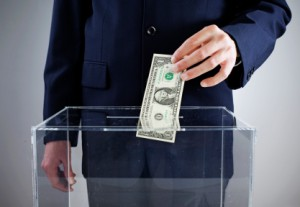
\includegraphics[width=0.45\textwidth]{images/moneyballot.jpeg}
    \end{figure}
    \vspace{2pt}
\end{center}
\begin{itemize}
\pause \item Economy's effect on the presidential election is clear
\pause \item A healthy economy boosts the chances of the incumbent candidate/party, while a weak economy lowers its chances
\end{itemize}
\end{frame}

%Problem - Election on Economy?
\begin{frame}
    \frametitle{Problem}
However, the effect of the presidential elections on the economy is not as clear.

Direct factors that affect the economy:
\begin{itemize}
\item Progressively more elaborate and expensive presidential campaigns
\end{itemize}

Indirect factors that affect the economy:
\begin{itemize}
 \item Policy deferment
 \item Political indecision
\end{itemize}

\begin{center}
    \begin{figure}
            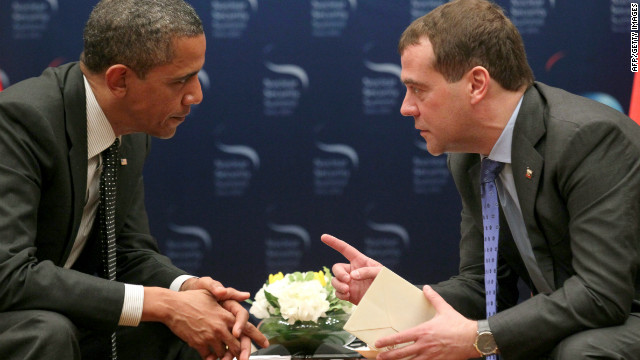
\includegraphics[width=0.45\textwidth]{images/obamamedvedev.jpeg}
    \end{figure}
\end{center}

\end{frame}

%Objective 
\section{Objective}
\begin{frame}
    \frametitle{Objective}
  {\large To quantify the economic effects of presidential elections/campaigns } 
\vspace{10pt}

\begin{itemize}
\item  To investigate if, during the period before and after historical presidential elections, there exists statiscally significant fluctuations that can be tied to events related to the presidential election (i.e. announcement of election results)
\end{itemize}
\end{frame}

%Approach 
\section{Approach}
\begin{frame}
    \frametitle{Approach}
\begin{center}
            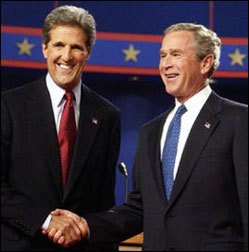
\includegraphics[width=0.2\textwidth]{images/2004election.jpeg}
\end{center}
\begin{itemize}
\item  2004 Presidential Election 
\item Two economic indicators:
	\begin{enumerate}
		\item S\&P 500 index
		\item Price of U.S. 1-year Treasury Bill
	\end{enumerate}
\item Data running from 1999 (5 years prior) to 2009 (5 years after)
\end{itemize}
\end{frame}


%other indicators
\begin{frame}
    \frametitle{Economic Indicators}

Numerous other indicators that can measure effects on the economy:
\begin{itemize}
    \item Gross Domestic Product (GDP)
    \item Unemployment Rate
    \item Consumer Price Index (CPI)
    \item Crude Oil Prices
    \item Gold Prices
\end{itemize}

\end{frame}

%S&P500
\begin{frame}
    \frametitle{The S\&P 500 Index}
\begin{center}
            
\includegraphics[width=0.25\textwidth]{images/SP500.jpeg}
\end{center}
\begin{itemize}
\item  Stock market index based on the common stock prices of 500 top publicly traded American companies, as determined by Standard \& Poor's
\item Index is updated every 15 seconds
\item Commonly regarded as a good representation of the market and an indicator for the U.S. economy
\end{itemize}
\end{frame}

%T-bills
\begin{frame}
    \frametitle{United States Treasury Bills}
\begin{center}
            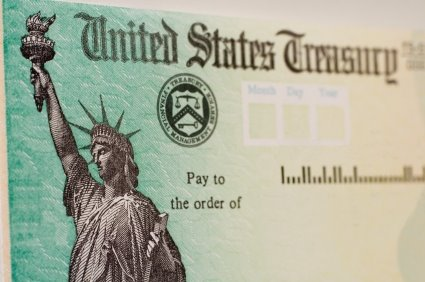
\includegraphics[width=0.25\textwidth]{images/ustreasury.jpeg}
\end{center}
\begin{itemize}
\item  U.S. 1-year Treasury Bills (`T-Bills') are short term loans issued to, and backed by the full faith and credit of, the United States Government
\item Regarded as the least risky investment available to U.S. investors
\item Price of these actively traded bills are also a good indicator of the confidence in the U.S. lending market, and the economy as a whole
\end{itemize}
\end{frame}

%Analyzing  data
\begin{frame}
    \frametitle{Analyzing economic indicators}
The S\&P 500 Index over 10 years:
\begin{center}
            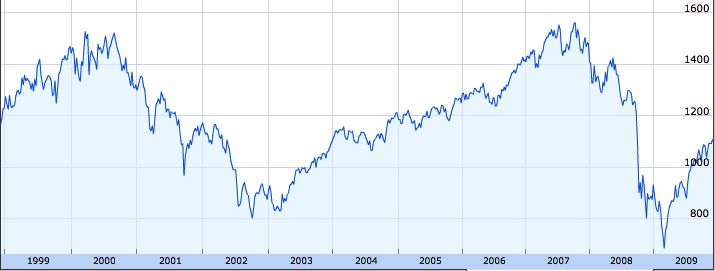
\includegraphics[width=0.75\textwidth]{images/SP500latest.png}
\end{center}

To test the effect of the conclusion of a presidential election against these economic indicators

\begin{enumerate}
\item Analyze daily fluctuations in the both indicators 5 years before and after the presidential election
\item Analyze the change in both indicators the day before election day, and the day after
\item Compare normalized historical fluctuations with fluctuations on election day
\end{enumerate}

\end{frame}

%Method
\begin{frame}
    \frametitle{Method: Change-point detection}


\begin{itemize}
\item The time series of these two indicators are analyzed using change-point detection

\item Change-points are times of discontinuities in a time series that can be induced from changes in observation

\item To what extent the presidential elections affect the economy.

\end{itemize}

\end{frame}

%Deliverables
\section{Deliverables}

\begin{frame}
\frametitle{Deliverables} 
The following outputs are expected from this project:
\begin{itemize}
    \item List of economic indicators 
    \item Statistical algorithm 
    \item R package with a complete set of documentations along with some test codes that can be used to reproduce our statistical test results
    \item Technical report and presentations summarizing the work
\end{itemize}

\end{frame}



%Deadlines / Progress / Work remaining
\section{Deadlines}
\begin{frame}
    \frametitle{Deadlines and Progress}

We have the following major deadlines:
\begin{itemize}
    \item Work Statement due date, Sep 28, 2012
    \item Data Acquisition due date, Oct 12, 2012
    \item Algorithm Design due date, Oct 26, 2012
    \item Midterm Presentation due date, Oct 26, 2012
    \item Progress Report due date, Nov 6, 2012
    \item Final Presentation due date, Nov 20, 2012
    \item Final Report due date, Nov 30, 2012
\end{itemize}

\end{frame}


%Future research 
\section{Future research}
\begin{frame}
    \frametitle{Future Research}

\begin{itemize}
    \item Analysis on other economic indicators previously discussed
    \item Analysis/research on the reliability of the stock market as an indicator (e.g. flash crash?)
	\item Localize analysis of political campaign's effect on an economy (by State / County)
\end{itemize}
\begin{center}
            
\includegraphics[width=0.3\textwidth]{images/campaign.jpeg}
\end{center}
\end{frame}


\end{document}

%http://www.treasury.gov/resource-center/data-chart-center/interest-rates/Pages/default.aspx
